\documentclass{amsart}
\usepackage{amsaddr}
\usepackage[style=numeric,backend=biber]{biblatex}
\addbibresource{paper.bib}

\usepackage{amsfonts}
\usepackage{amsmath}
\usepackage{amssymb}
\usepackage{amsbsy}
\usepackage{amsthm}
\usepackage{graphicx}
\usepackage{fancyhdr}
\usepackage{hyperref}
\usepackage[hypcap=true]{caption}
\usepackage{tikz}
\usepackage{siunitx}
\usepackage[english]{babel}
\usepackage{csquotes}
\usepackage{subcaption}
\usepackage{tabularx}
\usepackage{placeins}

%% Braces
\newcommand{\br}[1]{\left(#1\right)}
\newcommand{\brr}[1]{\left[#1\right]}

\newcommand{\dx}{\mathrm{d}x}
\newcommand{\dy}{\mathrm{d}y}
\newcommand{\dz}{\mathrm{d}z}
\newcommand{\dr}{\mathrm{d}r}
\newcommand{\dt}{\mathrm{d}t}
\newcommand{\ds}{\mathrm{d}s}
\newcommand{\dtau}{\mathrm{d}\tau}


%% Probability
\newcommand{\E}[1]{E\brr{#1}}

%% Functions
\newcommand{\fx}{f\left(x\right)}
\newcommand{\fnx}{f_n\left(x\right)}
\newcommand{\gx}{g\left(x\right)}
\newcommand{\gnx}{g_n\left(x\right)}
\newcommand{\hx}{h\left(x\right)}
\newcommand{\hnx}{h_n\left(x\right)}

\newcommand{\ff}[1]{f\left(#1\right)}
\newcommand{\ffd}[1]{f'\left(#1\right)}

\newcommand{\fg}[1]{g\left(#1\right)}

\newcommand{\ffn}[1]{f_n\left(#1\right)}
\newcommand{\ffnd}[1]{f_n'\left(#1\right)}
\newcommand{\ffndd}[1]{f_n''\left(#1\right)}


\newcommand{\ffk}[1]{f_k\left(#1\right)}
\newcommand{\ffkx}{f_k\left(x\right)}
\newcommand{\seriesfk}{\sum_{k=0}^{\infty}\ffkx}


\newcommand{\flog}[1]{\log\left(#1\right)}
\newcommand{\fexp}[1]{\exp\left(#1\right)}
\newcommand{\fsin}[1]{\sin\left(#1\right)}
\newcommand{\fcos}[1]{\cos\left(#1\right)}

\newcommand{\fabs}[1]{\left|#1\right|}


%% Common Spaces
\newcommand{\N}{\mathbb{N}}
\newcommand{\ZZ}{\mathbb{Z}}
\newcommand{\R}{\mathbb{R}}
%\newcommand{\Rn}{\R^n}
\newcommand{\CC}{\mathbb{C}}
\newcommand{\Q}{\mathbb{Q}}

%% sequences
\newcommand{\seq}[2]{\left(#1_{#2}\right)_{#2 \in \N}}
\newcommand{\seqxn}{\seq{x}{n}}
\newcommand{\seqxnk}{\left(x_{n_k}\right)_{k \in \N}}
\newcommand{\seqxk}{\seq{x}{k}}
\newcommand{\seqyn}{\seq{y}{n}}
\newcommand{\seqyk}{\seq{y}{k}}


%% Equations
\newcommand{\be}{\begin{equation*}}
\newcommand{\ee}{\end{equation*}}

\def\ba#1\ea{\begin{align*}#1\end{align*}}


%% Limits
\newcommand{\limn}{\lim_{n \to \infty}}
\newcommand{\limx}{\lim_{x \to \infty}}


%% Sets
\newcommand{\set}[1]{\left\{#1\right\}}

%% Series
\newcommand{\series}[2]{\sum_{n=#1}^{\infty} #2_n}

\newcommand{\seriesa}{\sum_{n=0}^{\infty} a_n}
\newcommand{\seriesb}{\sum_{n=0}^{\infty} b_n}


%% Misc
\newcommand{\setof}[1]{\left\{#1\right\}}

\DeclareMathOperator{\trace}{trace}

\DeclareMathOperator{\grad}{grad}
\DeclareMathOperator{\divop}{div}

%% theorems
\newtheorem{theorem}{Theorem}[section]
\newtheorem{lemma}[theorem]{Lemma}

\theoremstyle{definition}
\newtheorem{definition}[theorem]{Definition}
\newtheorem{example}[theorem]{Example}

\theoremstyle{remark}
\newtheorem{remark}[theorem]{Remark}

%% Normed spaces
\newcommand{\contfun}[1]{C\brr{#1}}

\newcommand{\fnorm}[1]{\left|\left| #1 \right| \right|}
\newcommand{\fnormp}[1]{\left|\left| #1 \right| \right|_p}
\newcommand{\fnormtwo}[1]{\left|\left| #1 \right| \right|_2}
\newcommand{\fnorminf}[1]{\left|\left| #1 \right| \right|_{\infty}}

\newcommand{\fscalar}[2]{\left\langle #1, #2 \right\rangle}
\newcommand{\fscalard}{\fscalar{\cdot}{\cdot}}
\newcommand{\seqfn}{\seq{f}{n}}


\numberwithin{equation}{section}

\begin{document}

\title{Fast Simulation of Multistage Clonal Expansion Models for Colorectal Cancer}

%    Remove any unused author tags.

%    author one information
\author{Lukas K\"ostler}
\email{lukas.koestler@tum.de}
\address{Technical University of Munich (TUM)}


%\keywords{Multistage Clonal Expansion, Filtered Poisson process}

\date{\today}


\begin{abstract}
We derive and demonstrate a method to simulate the Colorectal cancer model from \cite{jeon2008evaluation}. The method is faster than previous ones while retaining similar accuracy.
\end{abstract}

\maketitle


\section{Derivation}

\subsection{Poisson process with random start time}
We will consider a non-homogeneous Poisson process with rate $\lambda\br{t} > 0$ which has a random start time $\tau \geq 0$ with distribution $p$. For fixed $\tau$ the number of occurrences at time $t \geq \tau$ given start time $\tau$, $N\br{t} \vert \tau$ has the characteristic function \cite[chapter 4, eqn. (2.1)]{parzen1962stochastic}
\begin{align}\label{eqn:nonhompoisson}
\begin{split}
\varphi_{N\br{t} \vert \tau}\br{u} &= \exp\brr{m\br{t - \tau} \left\{e^{i u} - 1\right\}} \\
m\br{t} &= \int_0^t \lambda\br{s} \ds \, .
\end{split}
\end{align}
The by the law of total expectation, the characteristic function of $N\br{t}$ is given by
\begin{align*}
\varphi_{N\br{t}}\br{u} &= \E{\varphi_{N\br{t} \vert \tau}\br{u}} \\
&=\int_0^t \exp\brr{m\br{t - \tau} \left\{e^{i u} - 1\right\}} p \br{\tau} \, \dtau + \int_t^\infty p \br{\tau} \, \dtau \, .
\end{align*}
Comparing this expression to a Poisson process with different rate yields the first theorem.
\begin{theorem}\label{thm:iteratedpoisson}
Let $N\br{t}$ follow a non-homogeneous Poisson process with rate $\lambda\br{t} \geq 0$ starting at a random time $\tau \geq 0$ with probability density function $p\br{\tau}$. Let $M\br{t}$ follow a non-homogeneous Poisson process starting at time $0$ with rate
\begin{equation}
\nu\br{t} = \int_0^t\lambda\br{t-\tau} p\br{\tau} \ds = \br{\lambda \ast p}\br{t} \ .
\end{equation}
Then for the characteristic functions $\varphi_{N\br{t}}$ and $\varphi_{M\br{t}}$ there holds
\begin{equation}
\max_{t \in \brr{0, \sigma}} \fabs{\varphi_{N\br{t}} - \varphi_{M\br{t}}}
\leq 2 \br{\fexp{2 m\br{\sigma}} - 2m\br{\sigma} - 1}
= O (m\br{\sigma}^2) \,
\end{equation}
where $m$ is the mean value function of $N\br{t}$ as defined in eqn. \eqref{eqn:nonhompoisson}.
\end{theorem}
\begin{proof}
Let $h$ be the mean value function (eqn. \eqref{eqn:nonhompoisson}) of $M\br{t}$, then there holds
\begin{align*}
\frac{d}{dt} \int_0^t m\br{t - \tau} p\br{\tau} \dtau = \int_0^t m'\br{t - \tau} p \br{\tau} \dtau = \int_0^t\lambda\br{t-\tau} p\br{\tau} \dtau = \frac{d}{dt} \nu\br{t} \, .
\end{align*}
We used the Leibniz integration rule and $m\br{0} = 0$ in the first step. Because $h\br{0} = 0$ has to hold, we get
\begin{equation*}
h\br{t} = \int_0^t m\br{t - \tau} p\br{\tau} \dtau = \br{m \ast p}\br{t}
\end{equation*}\\

\noindent For $\varphi_{N\br{t}}\br{u}$, using $k := \left\{e^{i u} - 1\right\}$, we obtain
\begin{align*}
\varphi_{N\br{t}}\br{u}
&=\int_0^t \exp\brr{m\br{t - \tau} k} p \br{\tau} \, \dtau + \int_t^\infty p \br{\tau} \, \dtau \\
&= 1 + k \int_0^t m\br{t - \tau} p \br{\tau} \, \dtau + \sum_{j=2}^\infty \frac{k^j}{j!} \int_0^t m\br{t - \tau}^j p \br{\tau} \, \dtau \, .
\end{align*}\\

\noindent For $\varphi_{M\br{t}}\br{u}$ we obtain
\begin{align*}
\varphi_{M\br{t}}\br{u}
&= \fexp{h\br{t} k}
= 1 + k h\br{t} + \sum_{j=2}^\infty \frac{k^j}{j!} h\br{t}^j \, .
\end{align*}\\

\noindent Let $t \in \brr{0, \sigma}$ then there holds
\begin{align*}
\fabs{\varphi_{N\br{t}} - \varphi_{M\br{t}}}
&= \Big \vert \sum_{j=2}^\infty \frac{k^j}{j!} \int_0^t m\br{t - \tau}^j p \br{\tau} \, \dtau - \sum_{j=2}^\infty \frac{k^j}{j!} h\br{t}^j \Big \vert \\
&\leq \sum_{j=2}^\infty \frac{\fabs{k}^j}{j!} \Big\vert \int_0^t m\br{t - \tau}^j p \br{\tau} \, \dtau - \br{ \int_0^t m\br{t - \tau} p \br{\tau} \, \dtau }^j \Big\vert \\
&\leq \sum_{j=2}^\infty \frac{\fabs{k}^j}{j!} \br{\fabs{m\br{\sigma}}^j + \fabs{m\br{\sigma}}^j} \\
&=2 \sum_{j=2}^\infty \frac{\br{2 m\br{\sigma}}^j}{j!}\\
&=2 \br{\fexp{2 m\br{\sigma}} - 2m\br{\sigma} - 1} \, .
\end{align*}
We used that $\int_0^t p\br{\tau} \dtau = 1$ and that $m\br{\cdot}$ is positive and monotonically increasing.
\end{proof}

\begin{remark}
\autoref{thm:iteratedpoisson} is useful if $m\br{\sigma} \ll 1$ because it then implies that a Poisson process with random start time can be viewed (and simulated) as a Poisson process with rate $h = \br{m \ast p}$. This makes intuitive sense, because if $m\br{\sigma}$, i.e. the expected number of occurrences for $N\br{\sigma}$ starting at $0$, is much smaller than $1$ the correlation that is introduced through the random starting time is negligible.\\

\noindent The formulas for the mean and the variance are
\begin{align*}
\E{N\br{\sigma}} &= h\br{\sigma} \, ,\\
\E{M\br{\sigma}} &= h\br{\sigma} \, ,\\
Var\br{N\br{\sigma}} &= h\br{\sigma} + \int_0^\sigma m^2\br{t-\tau} p\br{\tau} \dtau - \br{\int_0^\sigma m\br{t-\tau} p\br{\tau} \dtau}^2 \, , \\
Var\br{M\br{\sigma}} &= h\br{\sigma} \, .
\end{align*}
While the mean is consistent, the difference in variance is of second order in $m$.
\end{remark}



\subsection{Two Stage Poisson Process}
We will consider a two stage Poisson process. The first process has rate $\nu\br{t}$ and each occurrence of the first process is the starting point of a second-stage process with rate $\lambda\br{t}$. We are interested in the number $N\br{t}$ of occurrences from the first process and the arrival times $u_j$ of the second-stage processes. It is vital that we do not need the arrival times of the first process.

\begin{theorem}\label{thm:twostagepoisson}
Let $N\br{t}$ be the number of occurrences of a non-homogeneous Poisson process with rate $\nu\br{t}$, mean value function $\eta\br{t}$ starting at time $0$. Let $u_1, \dots, u_{N\br{t}}$ denote the arrival times of this process.

For each $j = 1, \dots, N\br{t}$ let $Y\br{t, u_j}$ denote the number of occurrences of a non-homogeneous Poisson process with rate $\lambda\br{t}$, mean value function $m\br{t}$ starting at time $u_j$.

The process
\[
    Y\br{t} = \sum_{j=1}^{N\br{t}} Y\br{t, u_j}
\]{}
is called a filtered Poisson process \cite[chapter 4, eqn. (5.42)]{parzen1962stochastic}.
For $t \in \brr{0, \sigma}$, if we neglect terms of order $O(m\br{\sigma}^2)$:

\begin{enumerate}
% \item[i)] The process $Y\br{t}$ is a Poisson process with rate
% \[
%     \mu\br{t} = \br{\nu \ast \lambda}\br{t} \, .
% \]
\item[i)] Conditioned on $N\br{\sigma}$ the arrival times of the process $Y\br{t}$ follow a Poisson process with rate
\[
    \mu_{N}\br{t} = \frac{N\br{\sigma}}{\eta\br{\sigma}} \br{\nu \ast \lambda}\br{t} \qquad \forall t \in \brr{0, \sigma} \, .
\]
\end{enumerate}
\end{theorem}
\begin{proof}
By Proposition 2.206 in \cite[p. 147]{intro2015Stoch} (\emph{actually this only guarantees the property for a homogeneous process. I am quite certain that this also holds for the non-homogeneous case but I am lacking a source.}) we have that conditioned on $N\br{\sigma}$ the distribution for $u_j$ (note that the $u_j$ are not ordered) is given by $p\br{u} = \nu\br{u} / \eta\br{\sigma}$ and all $u_j$ are i.i.d.. Then we know by \autoref{thm:iteratedpoisson} that $Y\br{t, u_j}$ can be approximated up to order $2$ by a Poisson process with rate
\begin{equation*}
\mu_j\br{t} = \int_0^t\lambda\br{t-u} \frac{\nu\br{u}}{\eta\br{\sigma}} \mathrm{d}u = \frac{\br{\lambda \ast \nu}}{\eta\br{\sigma}} \br{t} \qquad \forall t \in \brr{0, \sigma} \, .
\end{equation*}
Because the sum of $N\br{\sigma}$ independent Poisson process is again a Poisson process, we know that $Y\br{t}$ can be approximated up to order $2$ by a Poisson process with rate
\[
    \mu_{N}\br{t} = \frac{N\br{\sigma}}{\eta\br{\sigma}} \br{\nu \ast \lambda}\br{t} \, .
\]{}
\end{proof}
\begin{remark}
\autoref{thm:twostagepoisson} is useful if $m\br{\sigma} \ll 1$ because it then implies that a two stage Poisson process can be simulated as follows. a) Draw $N\br{\sigma}$ at random from a Poisson distribution with mean $\eta\br{\sigma}$. b) Simulate a Poisson process with rate
\[
\frac{N\br{\sigma}}{\eta\br{\sigma}} \br{\nu \ast \lambda}\br{t} \, .
\]
The direct solution would be to simulate the first Poisson process fully and obtain arrival times $u_j$. For each arrival time one would simulate a Poisson process with rate $\lambda\br{t-u_j}$. This means on average $\eta\br{\sigma}$ many Poisson process simulations. The method proposed here can, under the circumstances described, generate a very good approximation with only two Poisson process simulations. This advantage comes from marginalizing out (approximately) the arrival times $u_j$.\\

\noindent For the Colorectal cancer model from \cite{jeon2008evaluation} the first rate is of order $10^2$, $\sigma=50$ and the second rate is of order $10^{-6}$. The direct approach results in approximately $5000$ Poisson process simulations. The approximate method yields a theoretic speedup factor of 1000. Also $m\br{\sigma} \approx 10^{-4}$ and thus the approximation extremely accurate.
\end{remark}


\newpage
\section{Numerical Experiments}
In this section we present numerical experiments for all theorems presented in this paper.

\subsection{Poisson process with random start time}
\label{sec:numPoissProcOne}
In Figure \ref{fig:numPoissProcOne} the model as described in \autoref{thm:iteratedpoisson} is simulated with a sample size of $10^7$. For $\lambda = 10^{-2}$ the approximation is already very accurate. The relative error in variance is $\lambda/6 \approx 1.7 \times 10^{-3}$ for $\lambda = 10^{-2}$.
\begin{figure}[ht]
    \centering
    \begin{subfigure}[t]{0.475\textwidth}
        \centering
        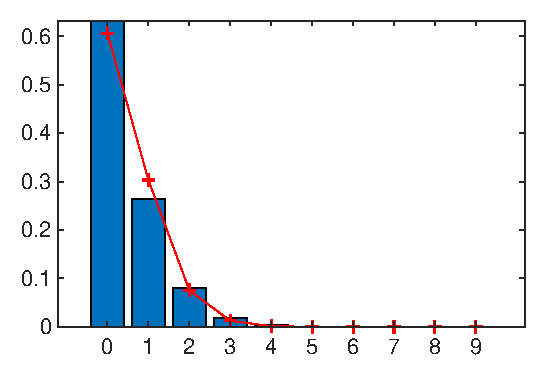
\includegraphics[width=\textwidth]{poissproc01_0_1.eps}
        \caption{$\lambda \equiv 1$}
    \end{subfigure}
    \hfill
    \begin{subfigure}[t]{0.475\textwidth}
        \centering
        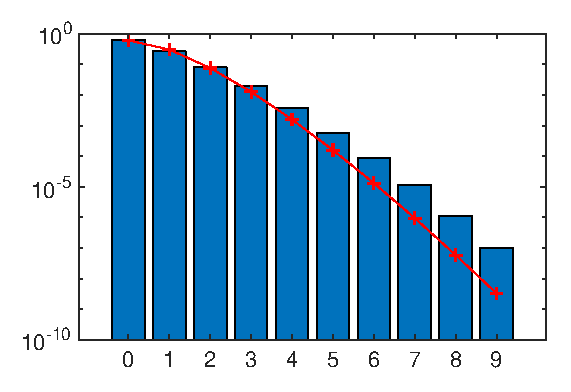
\includegraphics[width=\textwidth]{poissproc01_0_2.eps}
        \caption{$\lambda \equiv 1$. Log-Scale.}
    \end{subfigure}
    \\
    \begin{subfigure}[t]{0.475\textwidth}
        \centering
        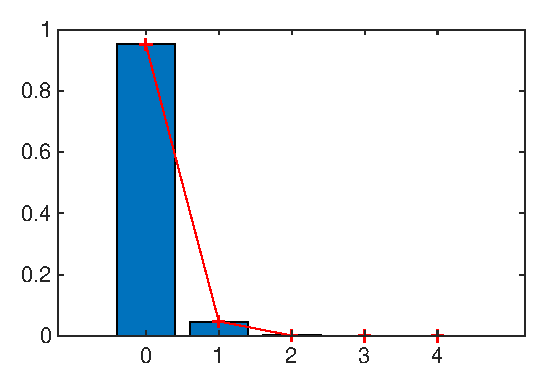
\includegraphics[width=\textwidth]{poissproc01_1_1.eps}
        \caption{$\lambda \equiv 10^{-1}$.}
    \end{subfigure}
    \hfill
    \begin{subfigure}[t]{0.475\textwidth}
        \centering
        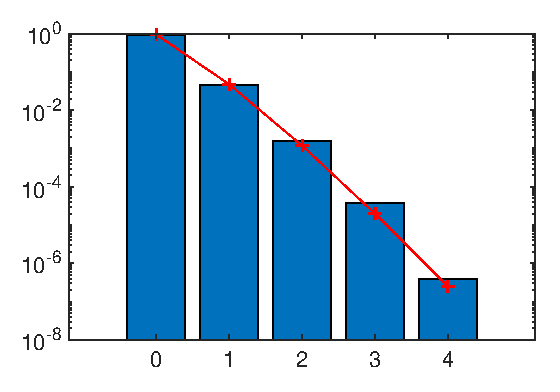
\includegraphics[width=\textwidth]{poissproc01_1_2.eps}
        \caption{$\lambda \equiv 10^{-1}$. Log-Scale.}
    \end{subfigure}
    \\
    \begin{subfigure}[t]{0.475\textwidth}
        \centering
        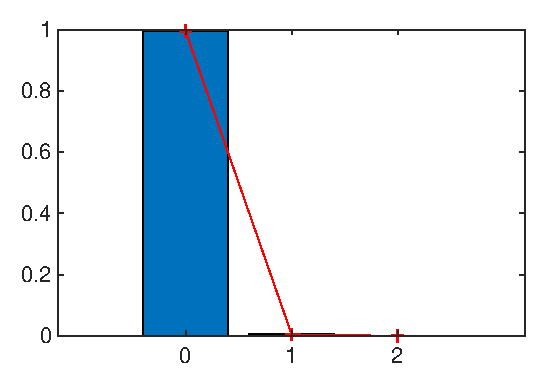
\includegraphics[width=\textwidth]{poissproc01_2_1.eps}
        \caption{$\lambda \equiv 10^{-2}$.}
    \end{subfigure}
    \hfill
    \begin{subfigure}[t]{0.475\textwidth}
        \centering
        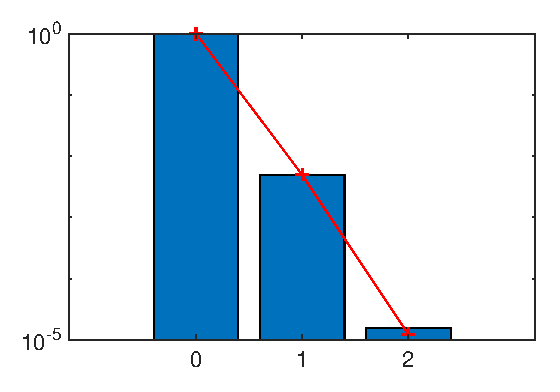
\includegraphics[width=\textwidth]{poissproc01_2_2.eps}
        \caption{$\lambda \equiv 10^{-2}$. Log-Scale.}
    \end{subfigure}
    \caption{$10^7$ samples. $\sigma = 1$. $\tau \sim \text{unif}\br{0,1}$. For this example there holds $\E{N} = \lambda / 2$ and $Var\br{N} = \lambda/2 + \lambda^2/12$}
    \label{fig:numPoissProcOne}
\end{figure}


\subsection{Two Stage Poisson Process}
\label{sec:numPoissProcTwo}


\newpage
\printbibliography
\end{document}
